%%%%%%%%%%%%%%%%%%%%%%%%%%%%%%%%%%%%%%%%%
% Stylish Article
% LaTeX Template
% Version 2.1 (1/10/15)
%
% This template has been downloaded from:
% http://www.LaTeXTemplates.com
%
% Original author:
% Mathias Legrand (legrand.mathias@gmail.com)
% With extensive modifications by:
% Vel (vel@latextemplates.com)
%
% License:
% CC BY-NC-SA 3.0 (http://creativecommons.org/licenses/by-nc-sa/3.0/)
%
%%%%%%%%%%%%%%%%%%%%%%%%%%%%%%%%%%%%%%%%%

%----------------------------------------------------------------------------------------
%	PACKAGES AND OTHER DOCUMENT CONFIGURATIONS
%----------------------------------------------------------------------------------------

\documentclass[fleqn,10pt]{SelfArx} % Document font size and equations flushed left

\usepackage[english]{babel} % Specify a different language here - english by default

\usepackage{lipsum} % Required to insert dummy text. To be removed otherwise
\usepackage{CJK}
%----------------------------------------------------------------------------------------
%	COLUMNS
%----------------------------------------------------------------------------------------

\setlength{\columnsep}{0.55cm} % Distance between the two columns of text
\setlength{\fboxrule}{0.75pt} % Width of the border around the abstract

%----------------------------------------------------------------------------------------
%	COLORS
%----------------------------------------------------------------------------------------

\definecolor{color1}{RGB}{0,0,90} % Color of the article title and sections
\definecolor{color2}{RGB}{0,20,20} % Color of the boxes behind the abstract and headings

%----------------------------------------------------------------------------------------
%	HYPERLINKS
%----------------------------------------------------------------------------------------

\usepackage{hyperref} % Required for hyperlinks
\hypersetup{hidelinks,colorlinks,breaklinks=true,urlcolor=color2,citecolor=color1,linkcolor=color1,bookmarksopen=false,pdftitle={Title},pdfauthor={Author}}

%----------------------------------------------------------------------------------------
%	ARTICLE INFORMATION
%----------------------------------------------------------------------------------------

\JournalInfo{Journal, Vol. XXI, No. 1, 1-5, 2013} % Journal information
\Archive{Additional note} % Additional notes (e.g. copyright, DOI, review/research article)

\PaperTitle{Article Title} % Article title

\Authors{John Smith\textsuperscript{1}*, James Smith\textsuperscript{2}} % Authors
\affiliation{\textsuperscript{1}\textit{Department of Biology, University of Examples, London, United Kingdom}} % Author affiliation
\affiliation{\textsuperscript{2}\textit{Department of Chemistry, University of Examples, London, United Kingdom}} % Author affiliation
\affiliation{*\textbf{Corresponding author}: john@smith.com} % Corresponding author

\Keywords{Keyword1 --- Keyword2 --- Keyword3} % Keywords - if you don't want any simply remove all the text between the curly brackets
\newcommand{\keywordname}{Keywords} % Defines the keywords heading name

%----------------------------------------------------------------------------------------
%	ABSTRACT
%----------------------------------------------------------------------------------------

\Abstract{\lipsum[1]~}

%----------------------------------------------------------------------------------------

\begin{document}
\begin{CJK}{UTF8}{gkai}

\maketitle % Print the title and abstract box
%----------------------------------------------------------------------------------------
%	ARTICLE CONTENTS
%----------------------------------------------------------------------------------------
%------------------------------------------------


\section{实验一}
\paragraph{问题描述}
问题描述:有限长序列x(n)=\[0,3,5,7,9,8,1,2,4,6\],按要求完成以下各小题
\subsection{求出它的DFT,请画出对应的幅度谱和相位谱;}
考虑到Matlab适合用于矩阵运算而非C语言式的下标寻址运算,所以考虑使用DFT的矩阵算法,即公式\ref{pro1_1}。
\begin{equation}
\left[\begin{array}{c}
X(0)\\
X(1)\\
\vdots\\
X(N-1)
\end{array}\right]
=
\left[\begin{array}{cccc}
1 & 1 & \cdots & 1\\
1 & W_N^1 \cdots & W_N^{N-1}\\
\vdots&\vdots&\ddots&\vdots\\
1 & W_N^{N-1} & \cdots & W_N^{(N-1)(N-1)}
\end{array}
\right]
\left[
\begin{array}{c}
  x(0)\\
  x(1)\\
  \vdots\\
  x(N-1)
\end{array}
\right]\label{pro1_1}
\end{equation}
观察公式\ref{pro1_1}中的DFT矩阵可得,该矩阵中的指数矩阵可由公式\ref{pro1_2}算出。
\begin{equation}
  \left[\begin{array}{cccc}
  0&0&\cdots&0\\
  0&1&\cdots&N-1\\
  \vdots&\vdots&\ddots&\vdots\\
  0&N-1&\cdots&(N-1)(N-1)
  \end{array}
  \right]
  =
  \left[\begin{array}{c}
  0\\
  1\\
  \vdots\\
  N-1
  \end{array}
  \right]
  \left[\begin{array}{cccc}
  0&1&\cdots&N-1
  \end{array}
  \right]\label{pro1_2}
\end{equation}
因此,该DFT算法流程为
\begin{enumerate}
  \item 求出输入向量长度
  \item 得到N维向量
  \item 求出指数矩阵
  \item 求出DFT矩阵
  \item 求出DFT结果
\end{enumerate}
算法运行结果如图\ref{pro1_fig1}
\begin{figure}
  \centering
  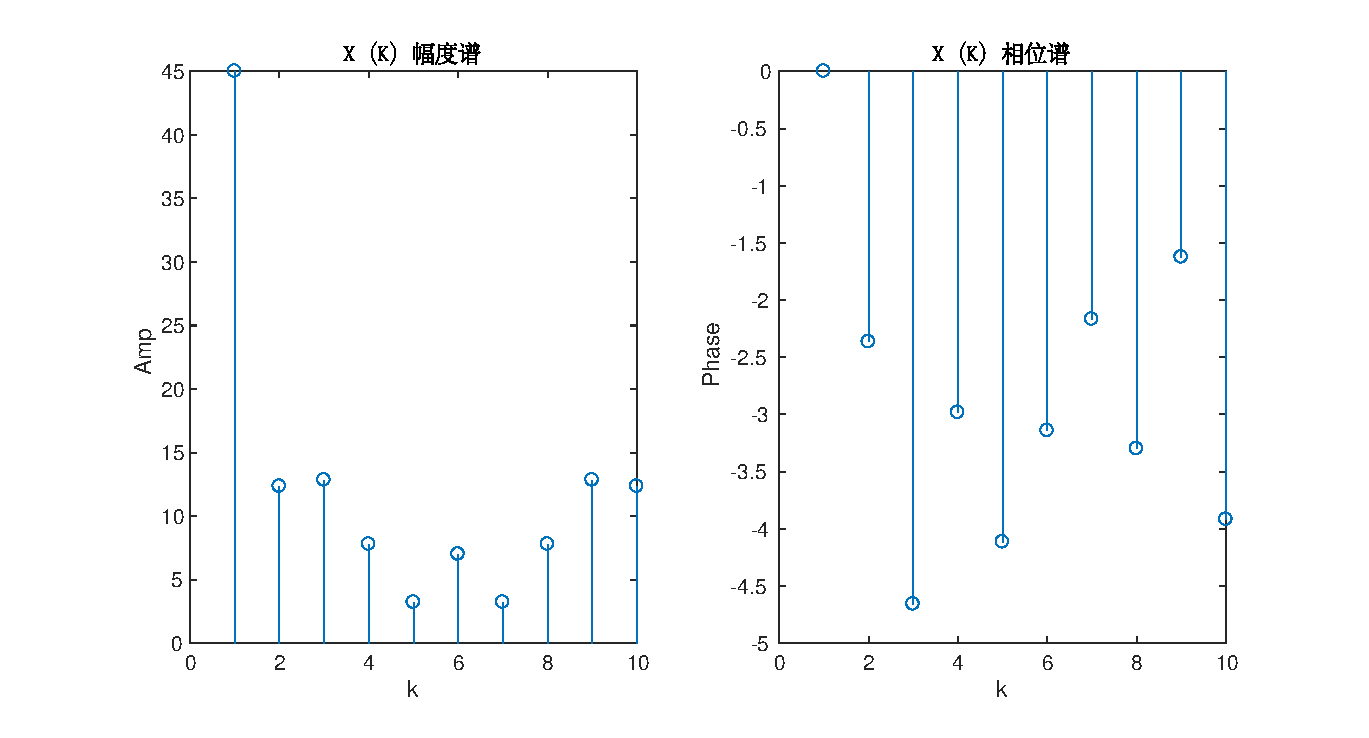
\includegraphics[scale=0.3]{pro1_subpro1.eps}
  \caption{输入信号DFT输出结果图}
  \label{pro1_fig1}
\end{figure}

\subsection{求它的IDFT,画出原信号与IDFT信号的对比图}
IDFT一样有矩阵算法,即公式\ref{pro1_3}
\begin{equation}
\left[\begin{array}{c}
x(0)\\
x(1)\\
\vdots\\
x(N-1)
\end{array}\right]
=
\frac{1}{N}
\left[\begin{array}{cccc}
1 & 1 & \cdots & 1\\
1 & W_N^{-1} \cdots & W_N^{-(N-1)}\\
\vdots&\vdots&\ddots&\vdots\\
1 & W_N^{-(N-1)} & \cdots & W_N^{-(N-1)(N-1)}
\end{array}
\right]
\left[
\begin{array}{c}
  X(0)\\
  X(1)\\
  \vdots\\
  X(N-1)
\end{array}
\right]\label{pro1_3}
\end{equation}
观察得出,其与DFT算法类似,只是指数矩阵需要求相反数,再乘上归一化常数即可。故此处不再赘述。IDFT结果如图\ref{pro1_fig2}和图\ref{pro1_fig3}。从图中可以看出,原信号和IDFT得到的信号不论是幅度,还是相位都相同,这也才符合DFT的基本要求。
\begin{figure}
  \centering
  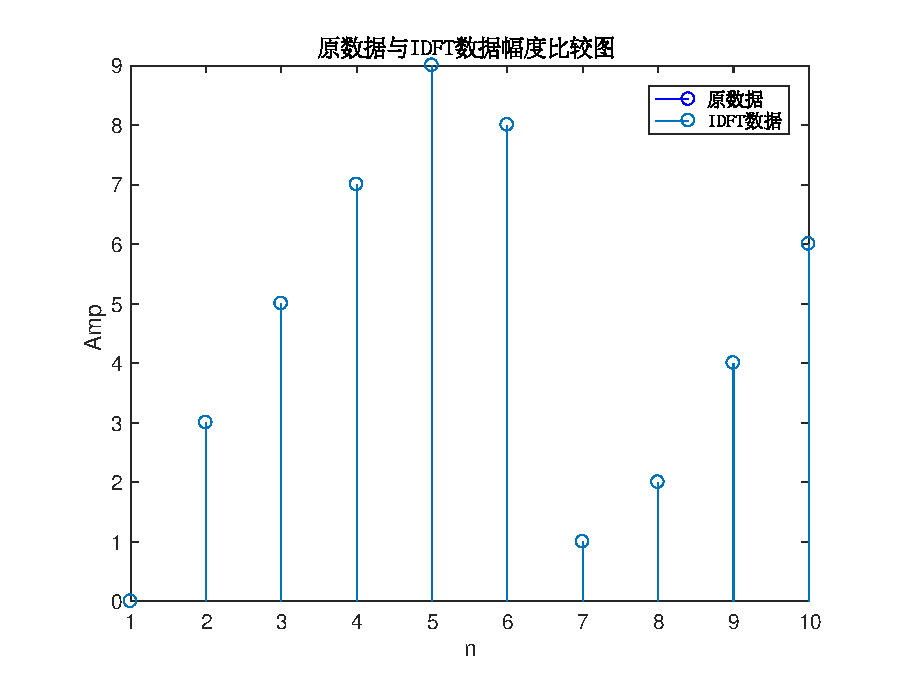
\includegraphics[scale=0.5]{pro1_subpro2_amp.eps}
  \caption{IDFT结果与原信号幅度对比图}
  \label{pro1_fig2}
\end{figure}
\begin{figure}
  \centering
  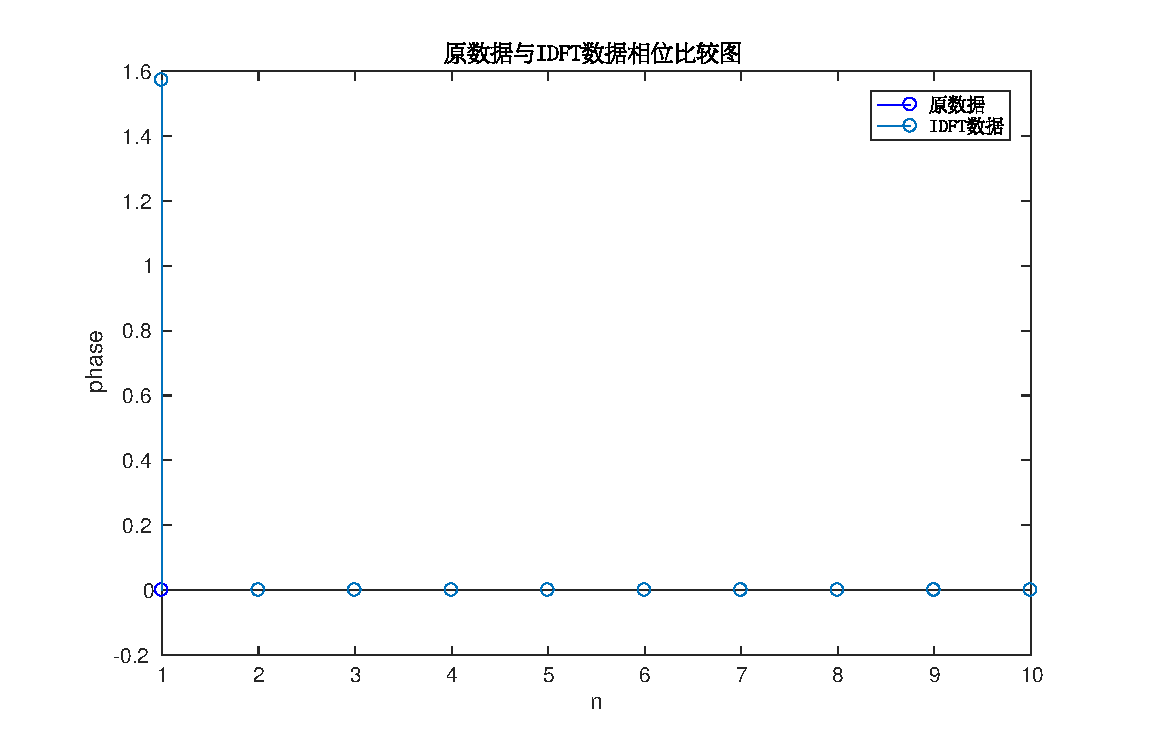
\includegraphics[scale=0.5]{pro1_subpro2_phase.eps}
  \caption{IDFT结果与原信号幅度对比图}
  \label{pro1_fig3}
\end{figure}
\subsection{在x(n)后面分别补10个0, 990个0,求新序列的DFT,并与原序列进行比较,解释不同}
按照题目要求,补0后再进行DFT运算得到的结果如图\ref{pro1_fig4}。从图中可以看出,对于幅度谱来说,补0后可以得到更高的分辨率,补的0越多分辨率越高,而不补0得到的结果也只是在补了很多0之后等间隔采样,最多也只是最后一个点因为函数连续性的问题而偏差较大,但也足够在相当的程度上反应该信号的幅度谱。\\
但对于相位谱却并不是如此,很容易可以看到,即使只是补了10个0的相位谱也已经和补了990个0的相位谱差别不大。然而不补0的序列DFT得到的相位谱却与之相差极大,这是因为相位具有每$2\pi$循环一周的特点,所以DFT求出的相邻两点间的相位差一直都位于$[-\pi,\pi]$的范围内。所以当频域采样间隔不够时,计算得到的结果就会将原本相位相差很多个$\pi$的结果取余数至$[-\pi,\pi]$也就不能反映真实的相位变化情况。因此,对于需要考虑某个信号相位谱的情况,必须进行补0操作再DFT,否则将无法合理判断出同相点和反相点所在位置。
\begin{figure}
  \centering
  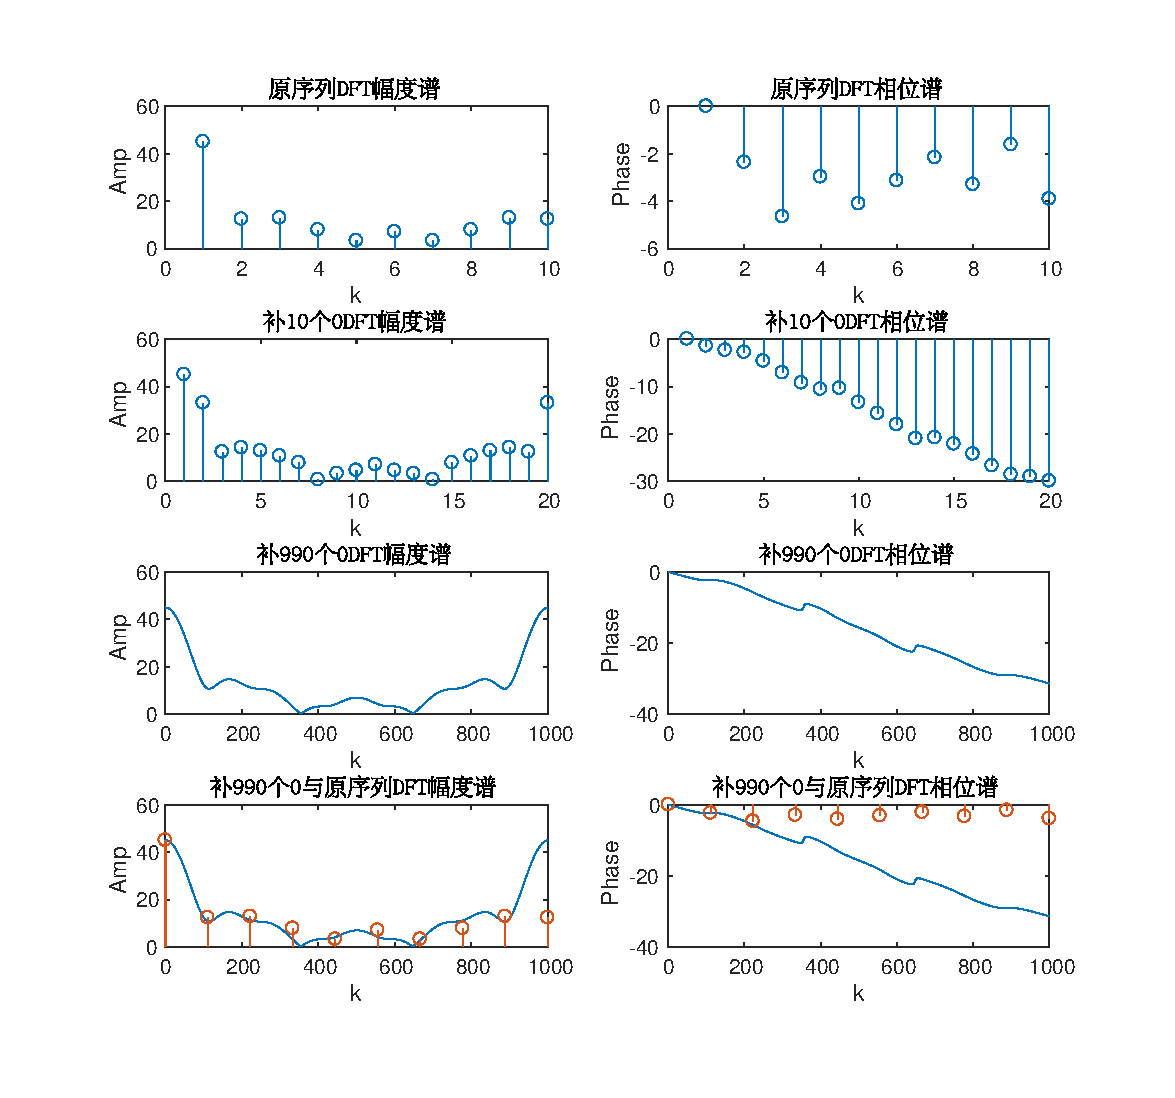
\includegraphics[scale=0.5]{pro1_subpro3.eps}
  \caption{序列补0DFT结果比较图}
  \label{pro1_fig4}
\end{figure}
\subsection{对x(n)进行8倍上采样(即每个点后面补7个0),求其DFT,并与原序列进行比较,解释不同}
为了实现起来比较简单,所以直接使用Matlab自带的upsample函数进行上采样操作,采样倍数选择8即可满足题目要求。再进行DFT计算后得到的结果如图\ref{pro1_fig5}和图\ref{pro1_fig6}。从这两幅图中可以看出,上采样后幅度谱被重复了8次 ,这使得噪声被平均分配到这八个谱上,然而我们只需要其中一个谱即可。所以这可以将噪声对传输的干扰减小到原来的$\frac{1}{8}$,极大地改善了传输效果。\\
观察相位谱可以发现,该相位谱也只是在周期重复,但由于DFT的相位差只能位于$[-\pi,\pi]$的范围内,所以出现了每重复一次相位差增加一个$2\pi$的情况,但又考虑到恢复信号的时候,相位谱不但只取八个谱中的一个,还要对$2\pi$取余,所以这些多出来的相位并不会对结果产生影响。\\
综上,八倍上采样可以将噪声对幅度谱和相位谱的影响都降低到原来的$\frac{1}{8}$,提高通信的质量。
\begin{figure}
  \centering
  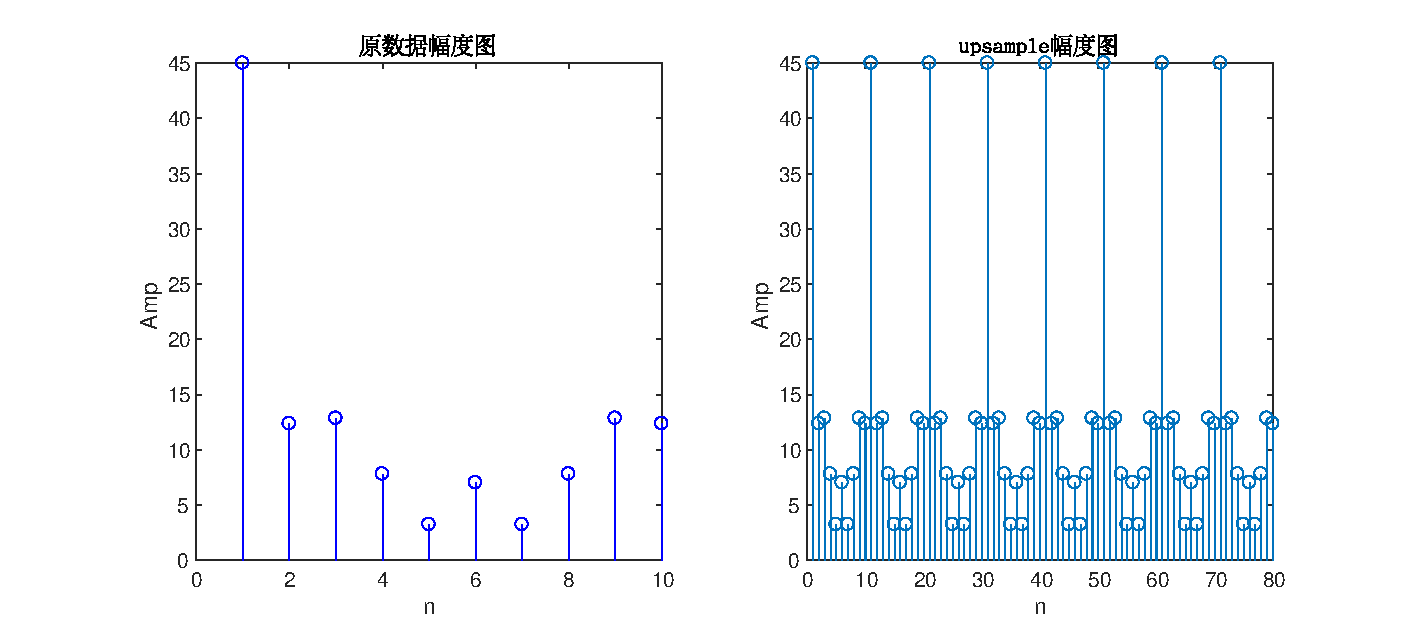
\includegraphics[scale=0.4]{pro1_subpro4_amp.eps}
  \caption{八倍上采样后的幅度谱}
  \label{pro1_fig5}
\end{figure}

\begin{figure}
  \centering
  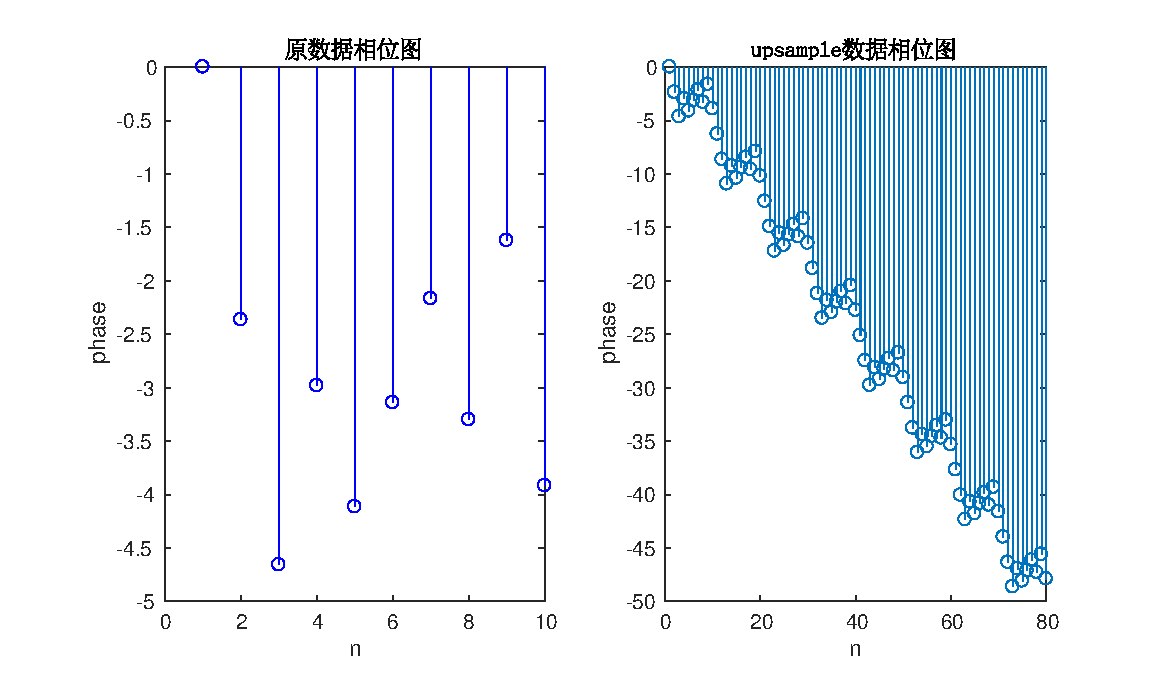
\includegraphics[scale=0.4]{pro1_subpro4_phase.eps}
  \caption{八倍上采样后相位谱}
  \label{pro1_fig6}
\end{figure}
\section{实验二}
问题描述:模拟信号$x_a=\sin(2\pi f_0t)+0.5\sin(6\pi f_0t),f_0=1Hz$,按要求完成以下各小题:
\subsection{分别设定采样频率为$5f_0$、$10f_0$、$15f_0$,绘制模拟信号图和采样后的离散信号图;(只需画出三个周期即可t:0—3)}
先生成采样间隔$10000f_0$的时间序列模拟出模拟信号的时域波形,再分别生成所需采样间隔的时间序列进行采样。得到的结果如图\ref{pro2_fig1}
\begin{figure}
  \centering
  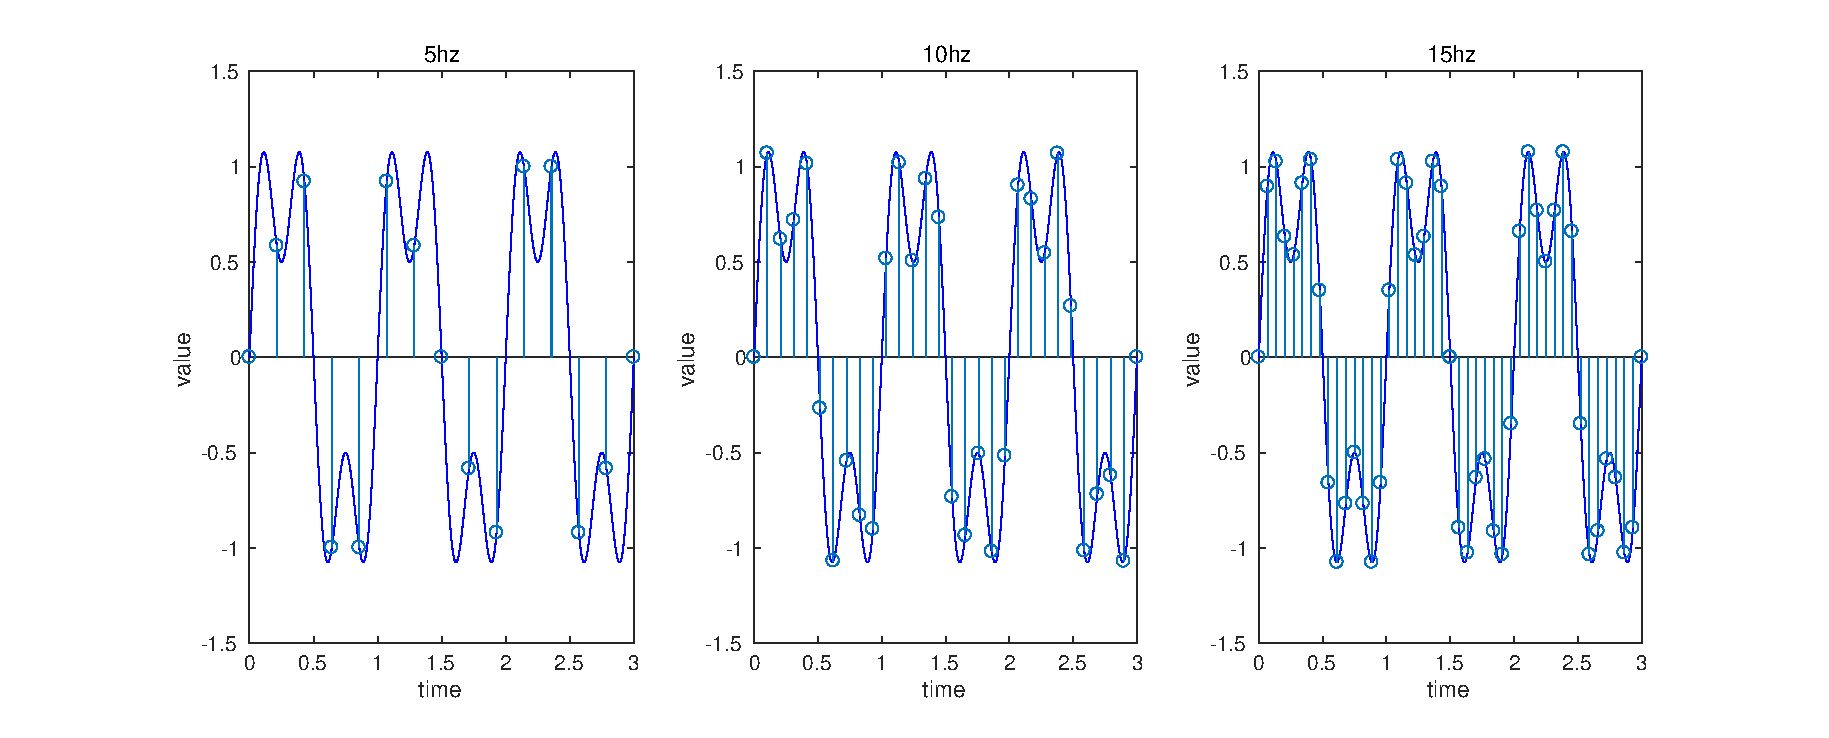
\includegraphics[scale=0.3]{pro2_subpro1.eps}
  \caption{不同采样率所得离散信号图谱}
  \label{pro2_fig1}
\end{figure}
\subsection{做FFT,画出其幅度谱,验证时域采样定理}
对三种时域采样得到的信号进行FFT可得幅度谱如图\ref{pro2_fig2}
\begin{figure}
  \centering
  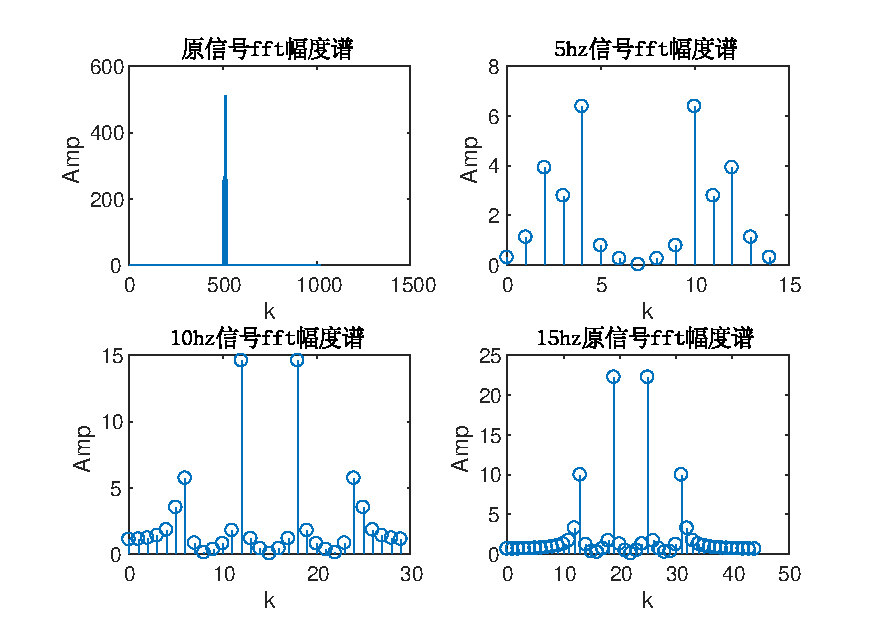
\includegraphics[scale=0.4]{pro2_subpro2.eps}
  \caption{不同采样率所得离散信号FFT幅度谱}
  \label{pro2_fig2}
\end{figure}
\begin{itemize}
  \item 原信号:原信号的频谱有两个峰,分别代表1Hz和3Hz的信号。此外,这两个峰的高度也反映了这两种信号的信号强度大小。
  \item 5Hz采样:该采样率下得到的FFT图谱只有一个峰,即5Hz采样只能完整采到1Hz的信号,并不能完整采到3Hz信号。
  \item 10Hz采样:该采样率已经高于信号最高频率3Hz的两倍,理论上能够完整采下3Hz的信号。FFT图谱中有两个峰,所以已经采到3Hz信号,但观察图谱边缘,可以发现边缘处的分量大小并没有明显趋于0。这表明该采样率下能够在一定程度上恢复原信号,但还是会有一定大小的失真。
  \item 15Hz采样:该采样率明显高于3Hz的两倍,FFT图谱中也出现了两个峰,而且边缘处信号分量也已经趋于0。所以,该采样率应该能够较好地恢复信号。
\end{itemize}

\subsection{用内插公式重建时域信号,并与原信号进行对比。}
将第二问中得到的三种FFT序列进行IFFT变换,得到还原信号的离散时间序列,再进行线性插值可得连续还原信号如图\ref{pro2_fig3}
\begin{figure}
  \centering
  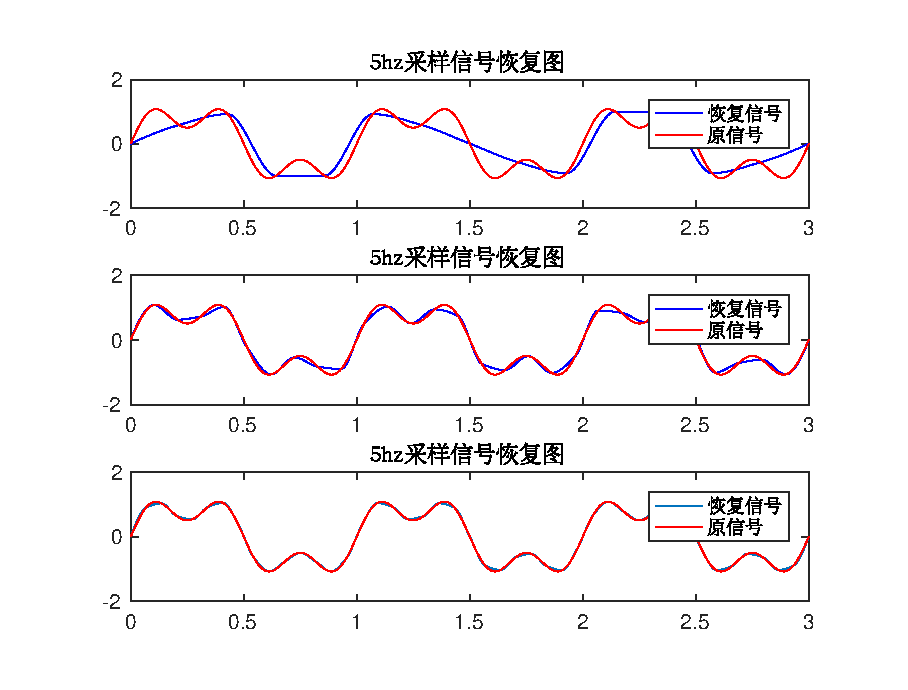
\includegraphics[scale=0.4]{pro2_subpro3.eps}
  \caption{不同采样率还原信号波形}
  \label{pro2_fig3}
\end{figure}
\begin{itemize}
  \item 5Hz采样率只恢复了信号的低频变化情况,缺少了很多信息。
  \item 10Hz采样率恢复了信号时域波形的大部分信息,但还是有一些小抖动。
  \item 15Hz采样率几乎完全恢复了原始信号。
\end{itemize}
综上,只有信号的采样率大于时域信号的最高频率的两倍才有可能完全恢复信号。但在实际的情况下,为了提高信号的恢复质量,需要适当提高采样率才能实现信号的无失真恢复。

\section{实验三}
问题描述:序列x(n)如\ref{pro3_equ1},按照以下要求完成下列各小题
\begin{equation}
  x(n)=\left\{
  \begin{array}{cc}
    n+1 & 0\leq n\leq13\\
    27-n & 14\leq n\leq26\\
    0 & other case
  \end{array}
  \right.
  \label{pro3_equ1}
\end{equation}
\subsection{绘制x(n)离散信号图,对进行1024点FFT,并图示之}
按照题目中所给的分段函数,可以得到该信号的时域离散信号图和1024点FFT变换如图
\begin{figure}
  \centering
  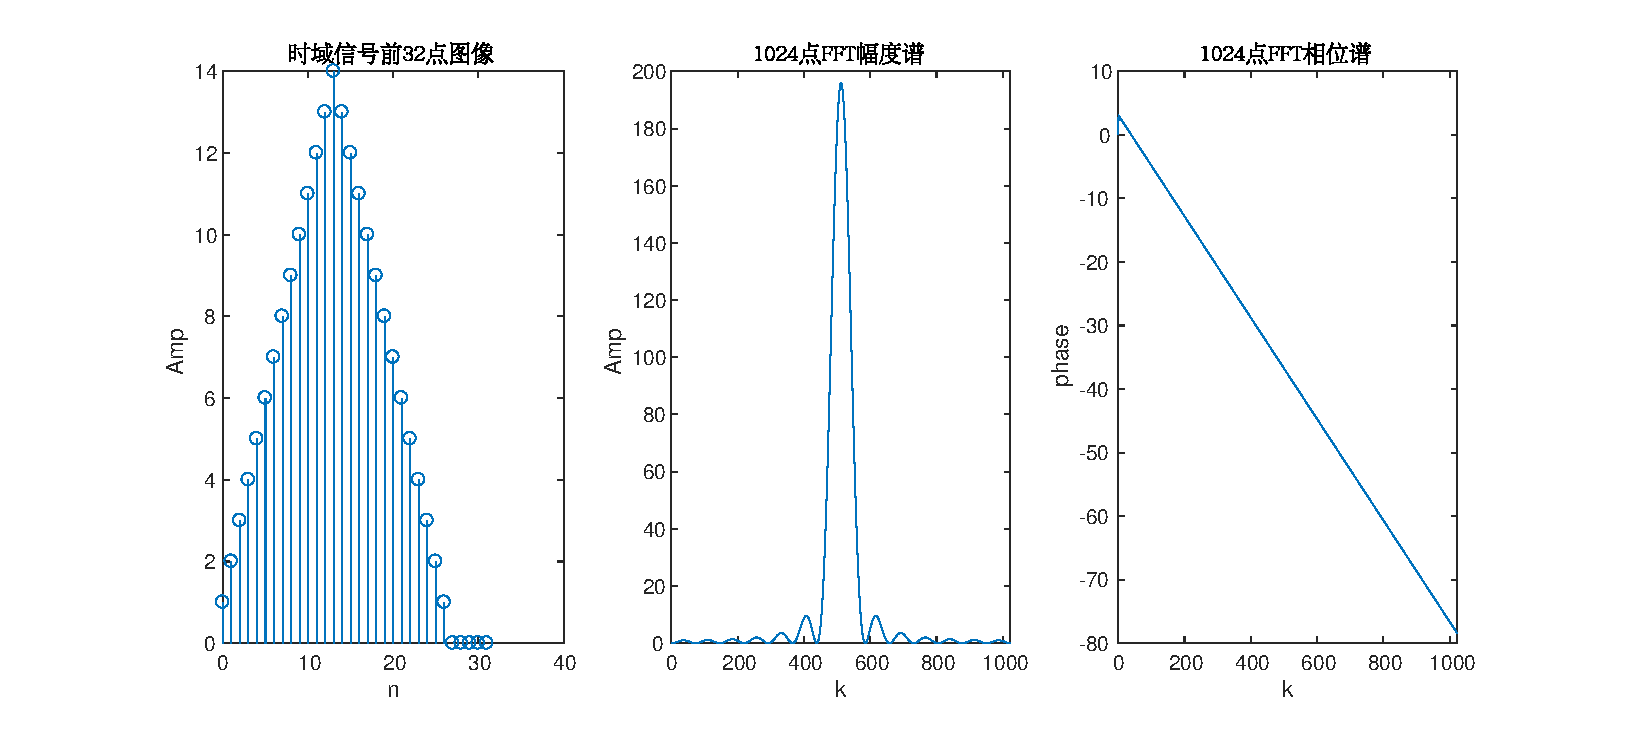
\includegraphics[scale=0.3]{pro3_subpro1.eps}
  \caption{原信号时域离散图和1024点FFT变换图}
  \label{pro3_fig1}
\end{figure}
\subsection{对x(n)进行N点FFT和IFFT,分别选取N>27和N<27, 对其进行FFT和IFFT,作图并验证频域采样定理}
对x(n)分别进行16点和32点FFT,再将其进行27点IFFT恢复原始波形如图\ref{pro2_fig2}。
\begin{figure}
  \centering
  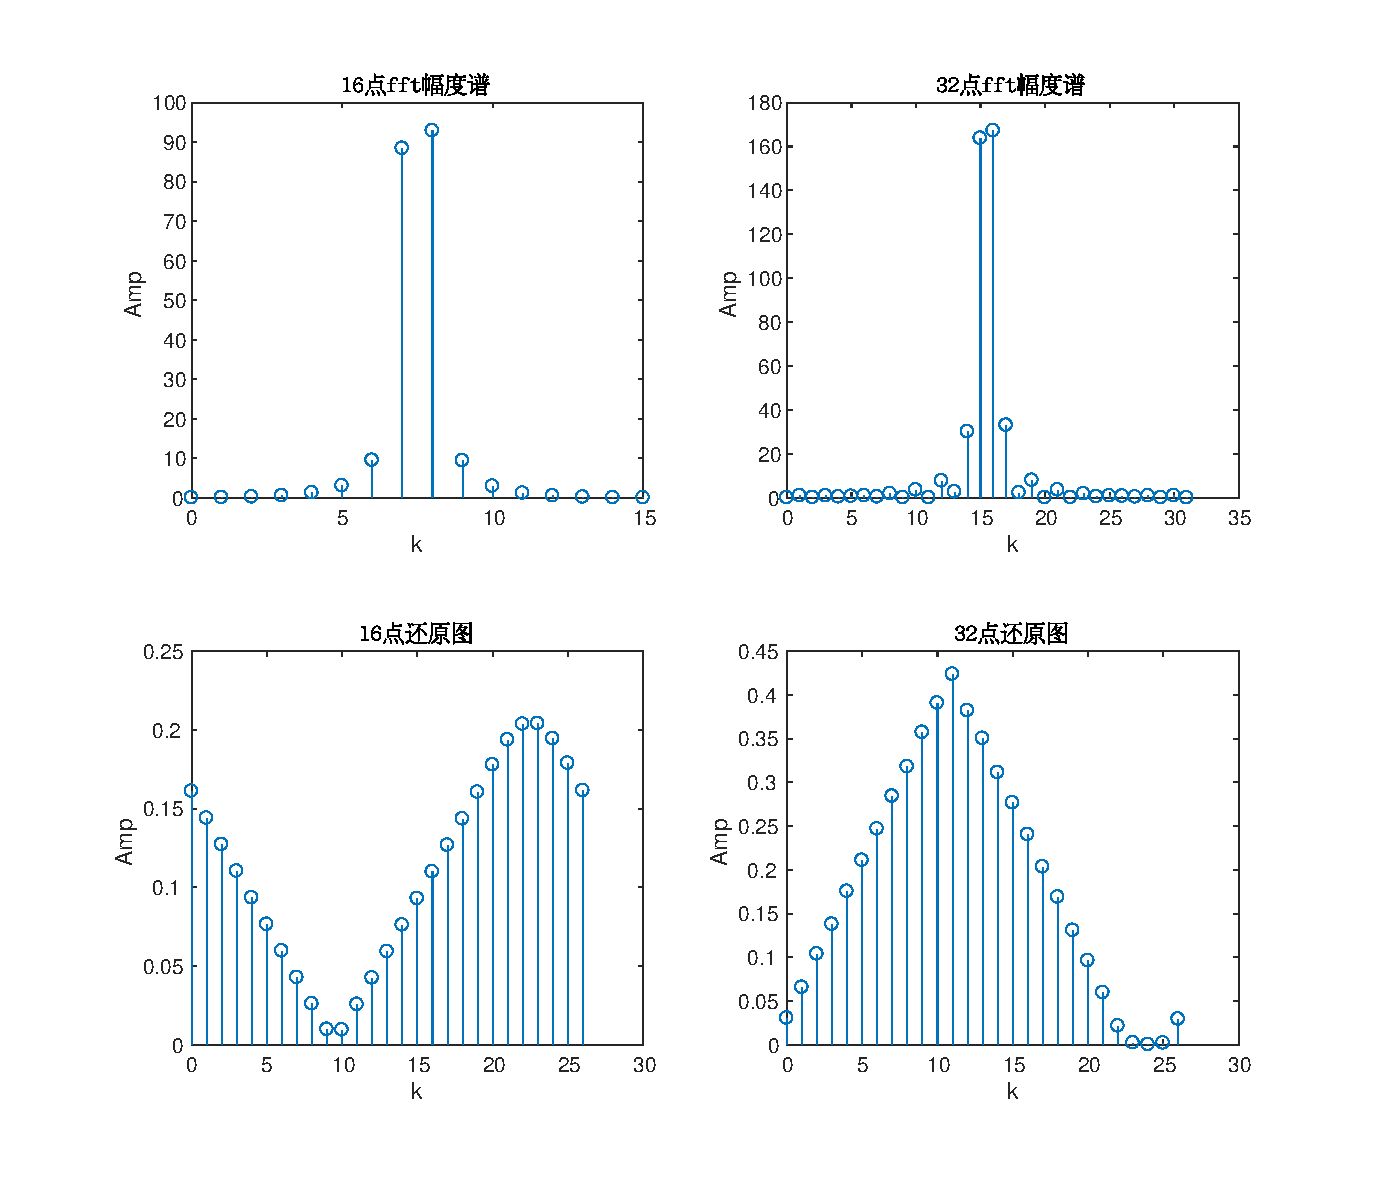
\includegraphics[scale=0.3]{pro3_subpro2_ifft.eps}
  \caption{16点/32点FFT和IFFT波形图}
  \label{pro3_fig2}
\end{figure}
\begin{figure}
  \centering
  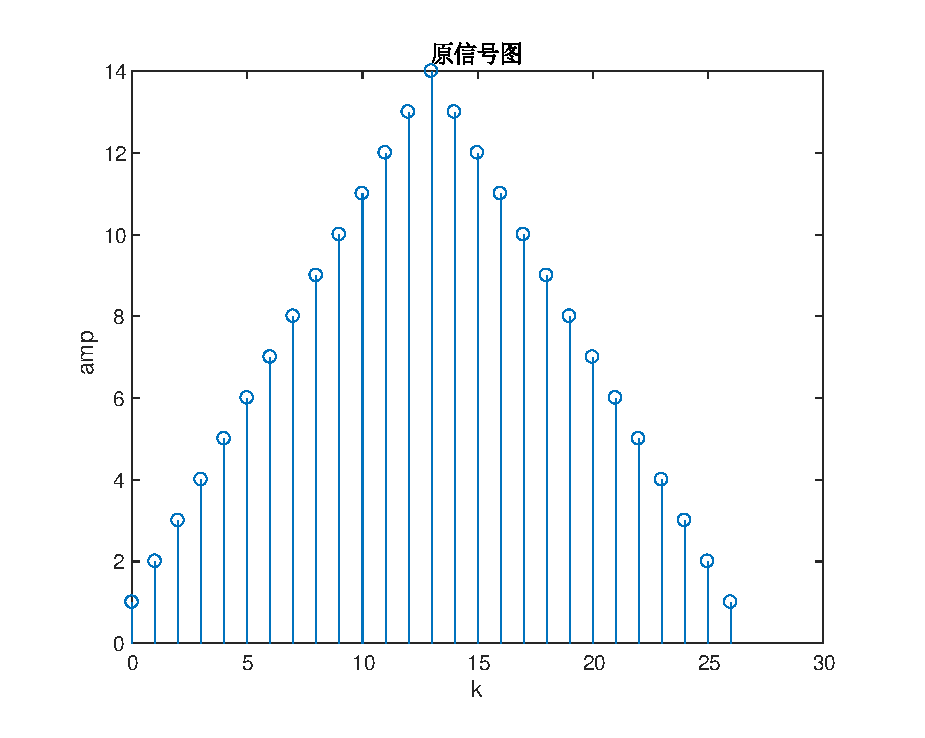
\includegraphics[scale=0.3]{pro3_subpro2_src.eps}
  \caption{原信号波形图}
  \label{pro3_fig3}
\end{figure}
与原信号图\ref{pro3_fig3}进行比较可以看到,由于16点FFT不满足频域采样定理,所以并不能恢复到27点时域波形。\\
而32点采样满足频域采样定理,所以可以较好地恢复27点时域波形。
\section{实验四}
问题描述:两组有限长序列x1(n)=[1 3 5 3 6 8 3 9],x2(n)=[2 3 4 6 7 9 0 2],计算两序列的圆周卷积y1(n)与线性卷积y2(n),比较二者的区别。\\\\
对两序列直接进行8点圆周卷积可得序列\ref{pro4_cir1}。
\begin{equation}
  \label{pro4_cir1}
\end{equation}
对两序列进行20点圆周卷积可得序列\ref{pro4_cir2}
\begin{equation}
  \label{pro4_cir2}
\end{equation}
对两序列进行线性卷积可得序列\ref{pro4_lin1}
\begin{equation}
  \label{pro4_lin1}
\end{equation}
比较两种圆周卷积方法得到的结果很容易发现,由于圆周卷积具有相位重复的特点,所以较短长度的圆周卷积会发生明显的混叠,与线性卷积相去甚远。而长度大于两信号长度和的圆周卷积结果则与线性卷积一致,只是需要进行相应的补零操作即可。\\
综上,只需要将离散输入信号进行相应地补零操作,再进行圆周卷积,就可以得到相应的线性卷积,方便了我们的计算。

\end{CJK}
\end{document}
